\documentclass[10pt]{article}
\usepackage[final]{graphicx}
\usepackage{amsfonts}
\usepackage{mathtools}
\usepackage{amsmath,amsthm,amssymb}
\usepackage{subcaption} 

\topmargin-.5in
\textwidth6.6in
\textheight9in
\oddsidemargin0in

\def\ds{\displaystyle}
\def\d{\partial}

\begin{document}

\centerline{\large \bf Title of Report}

\vspace{.1truein}

\def\thefootnote{\arabic{footnote}}
\begin{center}
  Author 1\footnote{Department, University},
  Author 2\footnote{Department, University},
  Author 3\footnote{Department, University},
  Author 4\footnote{Department, University},
  Author 5\footnote{Department, University}
\end{center}
\def\PM{{\mathrm{PM_{2.5}}}} 

%\vspace{.1truein}

\begin{center}
Faculty Mentors: Mentor 1\footnote{Company},
Mentor 2\footnote{University}
\end{center}


\vspace{.3truein}
\centerline{\bf Abstract}



\section{Computational Experiments}
Give enough details so that readers can duplicate your experiments.

\begin{itemize}
\item Describe the precise purpose of the experiments, and what they 
are supposed to show.

Our main goal is to explore the relationship between $\PM$ measurements obtained from the ground sites and the AOD measurements obtained from the satellite near the coast. We want to ascertain whether satellite remote sensing can be used to assess $\PM$ air quality for areas where surface $\PM$  monitors are not available. The AOD measurements reflect the integrated amount of particles in the vertical column, and can be used as an input parameter in statistical models for predicting $\PM$ levels. Since time-varying parameters such as relative humidity, wind direction, wind speed and air temperature can influence the $\PM$-AOD relationship, we want to formulate a statistical model that allows for day-to-day variability in this relationship.  \\

An appropriate initial model structure would probably involve modeling $\PM$ as a linear/non-linear function of the AOD measurements and other aforementioned time-varying parameters,but before attempting to fit the models, it is worth examining the data itself to look for possible problems. When this is done, AOD measurements with values $< -0.05$ appear problematic since AOD values are usually constrained to lie between 0 and unity. For this reason, these values are excluded from the analysis. \\ 

\begin{figure}[h]
\centering
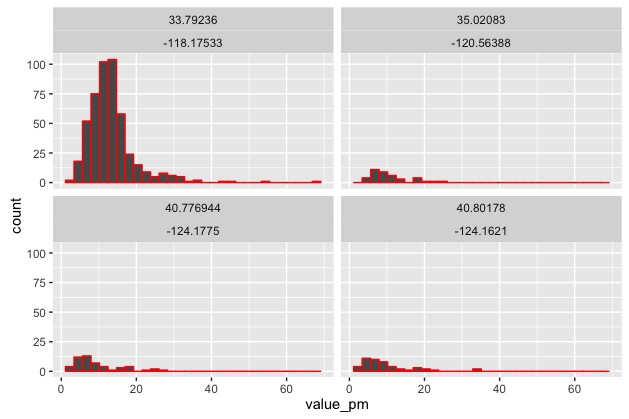
\includegraphics[width=100mm]{histpmcali.jpeg}
\caption{Histograms for $\PM$ measurements at 4 sites in California. The titles on each subpanel represent the latitudes and longitudes for the sites respectively.}
\end{figure}

The fairly skewed nature of the $\PM$ measurements, the response, and the fact that it is necessarily a positive quantity, suggest that some transformation maybe required if a Gaussian error model is to be used. Attempting to use a Gaussian model without transformation confirms this. The upper left normal QQ plot, in Figure, clearly shows a problem with the Gaussian assumption. Examining the plot on upper right of residuals versus fitted values reveals that the constant variance assumption is unreasonable. The lower left histogram of residuals confirms the pattern evident in the QQ plot: there are too many residuals in the lower tail which means that we tend to over estimate the $\PM$ levels using the model. The lower right plot emphasizes the failure of the constant variance assumption. \\ From figure 2, it is difficult to guess the appropriate transformation on the $\PM$ measurements that would alleviate this issue. We explored two options. Fitting the log transformation of the $\PM$ variable to the data tell the same story and, as before, runs into similar problems like non-constant variance and an unreasonable Gaussian assumption. The residual plots are not shown here. \newpage

\begin{figure}[h]
\centering
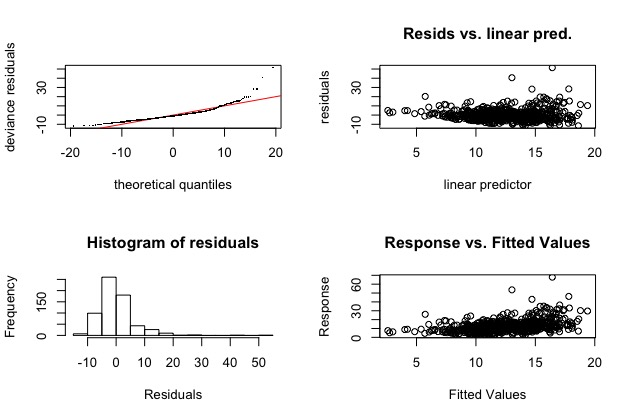
\includegraphics[width = 100mm]{gauss_diag.jpeg} 
\caption{Some basic model checking plots for a model fitted to the $\PM$ - AOD data} 
\end{figure}

Taking cue from (cite paper), we model the variabilities in $\PM$ concentrations using generalized additive models (GAMSs) (Hastie and Tibsirani 1990). Our model can be described as follows, 
\begin{equation} 
Y_{t,site} = \mu + \text{AOD} + f_{U,V}(U,V) + f_{H}(H) + f_{temp}(temp) + \text{Season} +  \epsilon, \;\; \epsilon ~ \text{Gamma}
\end{equation} 
$Y_{t, \text{site}}$ is the daily $\PM$ concentration at a given site. All the covariates (right hand side of the equation 1) vary with time and site. $\mu$ is the random model intercept, $f_{U,V}(U,V)$ is a two-dimensional smooth surface describing the impact of wind speed and direction on the AOD-$\PM$ association. Season is modeled as a 4-level categorical variable because of its discrete values. We fit the model with the $gam()$ function in the {\textit{mgcv}} package in R (Wood 2006). We represented the one-dimensional smooth terms such as $f_{H}(H)$ and $f_{temp}(temp)$ by penalized cubic splines to begin with. (Note: We need to try other options as well.)

\underline{Results for the model above} 
\begin{figure}[h]
\centering 
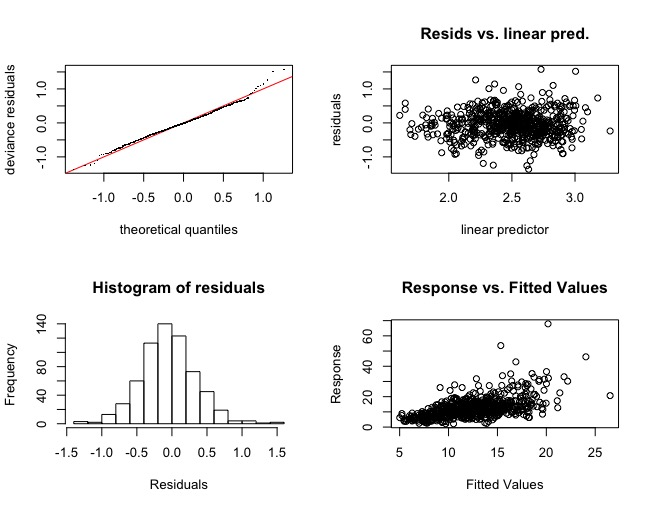
\includegraphics[width = 100mm]{cali_diag.jpeg}
\caption{Model diagnostics for model 1}
\end{figure}

\begin{figure}[h]
\centering
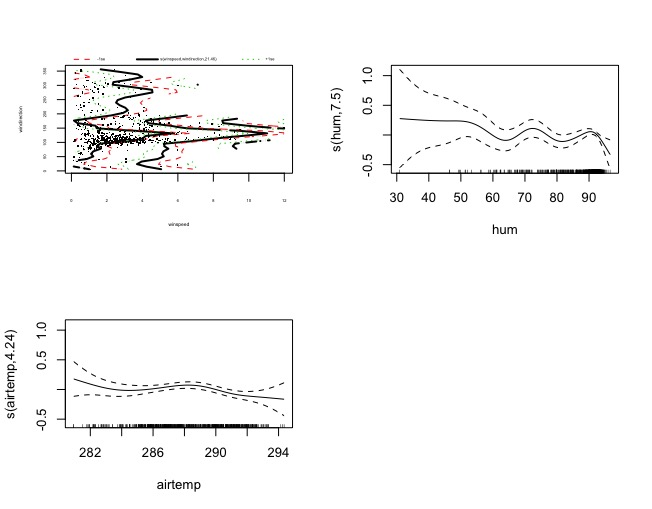
\includegraphics[width = 90mm]{cov_splines.jpeg} 
\caption{The estimates of the smooth functions shown without partial residuals. The dotted lines aound the solid lines show the Bayesian credible intervals.} 
\end{figure} 
\begin{verbatim} 
Family: Gamma 
Link function: log 

Formula:
value_pm ~ (value_aod) + s(winspeed, windirection) + s(hum) + 
    s(airtemp) + season

Parametric coefficients:
            Estimate Std. Error t value Pr(>|t|)    
(Intercept)   2.1283     0.0538   39.59  < 2e-16 ***
value_aod     0.3666     0.1579    2.32    0.021 *  
season        0.1386     0.0196    7.06  4.8e-12 ***
---
Signif. codes:  0 ‘***’ 0.001 ‘**’ 0.01 ‘*’ 0.05 ‘.’ 0.1 ‘ ’ 1

Approximate significance of smooth terms:
                           edf Ref.df    F p-value    
s(winspeed,windirection) 21.46  25.55 8.11  <2e-16 ***
s(hum)                    7.50   8.41 1.95   0.044 *  
s(airtemp)                4.24   5.26 2.56   0.024 *  
---
Signif. codes:  0 ‘***’ 0.001 ‘**’ 0.01 ‘*’ 0.05 ‘.’ 0.1 ‘ ’ 1

R-sq.(adj) =  0.266   Deviance explained = 36.2%
GCV = 0.17517  Scale est. = 0.17318   n = 630
\end{verbatim} 

$R^2 = .266$ is low since this analysis has been conducted for 4 sites in California. The cross-validation error is not too bad either. These values significantly improve considerably when we consider one site at a time. Doing an analysis of variance on the model (see below) shows that the two variables that significantly affect the $\PM$ levels are temperature and wind velocity. \newpage


%\begin{figure}[h]
%\centering
%\begin{subfigure}{.5\textwidth}
%\centering
%\includegraphics[width = .4\linewidth]{hist_hawa.jpeg}
%\caption{$\PM$ concentrations from 9 ground monitoring sites}
%\label{histpm}
%\end{subfigure}	
%\begin{subfigure}{.4\textwidth}
%\centering
%\includegraphics[width = .5\textwidth]{histaod_hawa.jpeg}
%\caption{AOD measurements from the satellite} 
%\end{subfigure}
%\caption{Histograms of the measurements at 9 sites in Hawaii} 
%\end{figure} 






\end{itemize}





\end{document}